%\setvruler[][][][3][0][1.2\textwidth]
\pagewiselinenumbers

\chapter{Introduction}
\pagenumbering{arabic}
\setcounter{page}{1}

This document defines the {\XMP} specification, which is a
directive-based language extension of {\Fort} and {\C} for scalable and
performance-aware parallel programming.
%
The specification includes a collection of compiler directives and
intrinsic and library procedures, and provides a model of parallel
programming for distributed memory multiprocessor systems.

%This document specifies a collection of compiler directives and runtime
%library routines that can be used to write distributed-memory parallel
%programs in {\C} and {\Fort}.These compiler directives define the
%specifications of the {\XMP} Application 
%Program Interface ({\XMP} API). These specifications provide a
%model of parallel programming for distributed memory multiprocessor
%systems. The directives extend the {\C} and {\Fort} base languages to
%describe distributed memory parallel programs.

\section{Features of {\XMP}}

The features of {\XMP} are summarized as follows:

\begin{itemize}

 \item {\XMP} supports typical parallelization based on the
       data-parallel paradigm and work mapping under the ``global-view''
       programming model, and it enables the parallelization of the
       original sequential code using minimal modification with simple
       directives such as {\OMP} \cite{omp}. Many ideas on ``global-view''
       programming are inherited from High Performance Fortran ({\HPF})
       \cite{hpf}.

 \item The important design principle of {\XMP} is
       ``performance-awareness.'' All actions related to communication
       and synchronization are taken by directives (and coarray features),
       which is different from automatic parallelizing compilers. The
       user should be aware of the effect of the {\XMP} directives in
       the execution model for distributed-memory architecture.

 \item {\XMP} also includes features from Partitioned Global Address
       Space (PGAS) languages, such as coarray of the {\Fort} 2008
       standard, for ``local-view'' programming.

 \item An extension of existing base languages with directives is useful
       to reduce code-rewriting and education costs. The {\XMP} language
       specification is defined as an extension to the {\Fort} and {\C}
       base languages.

 \item For flexibility and extensibility, the execution model enables us
       to combine {\XMP} with explicit Message Passing Interface ({\MPI})
       \cite{mpi} coding for more complicated and tuned parallel codes
       and libraries.

 \item For multi-core and SMP clusters, {\OMP} directives can be
       combined into {\XMP} for thread programming inside each node as a
       hybrid programming model.

% \item {\bf Language extensions} for familiar languages, such as {\C}
%       and Fortran, which can reduce code-rewriting and educational
%       costs.
%
% \item {\XMP} supports typical parallelization based on the {\bf data
%       parallel paradigm} and work sharing under {\it global view} and
%       enables parallelization of the original sequential code with
%       minimal modification using simple {\bf directives}, such as
%       {\OMP}.
%
% \item {\XMP} also includes a CAF-like Partitioned Global Address Space
%       (PGAS) feature as {\it local-view} programming.
%
% \item {\bf Explicit communication and synchronization}. All actions are
%       taken by directives for being ``easy-to-understand'' for
%       performance-aware programming
%
% \item For flexibility and extensibility, the execution model allows
%       {\bf combination with explicit {\MPI} coding} for more
%       complicated and tuned parallel codes and libraries.
%
% \item For multi-core and SMP clusters, {\bf {\OMP} directives can be
%       combined} into {\XMP} for thread programming inside each node as
%       a hybrid programming model.

\end{itemize}

{\XMP} is being designed based on experiences gained during the
development of HPF, HPF/JA \cite{hpfja}, Fujitsu XPF (VPP
FORTRAN) \cite{XPF,VPPFORTRAN}, and OpenMPD \cite{OpenMPD}.

\section{Scope}

The {\XMP} specification covers only user-directed parallelization,
where the user explicitly specifies the behavior of the compiler and
the runtime system in order to execute the program in parallel in a
distributed-memory system.
%
{\XMP}-compliant implementations are not required to automatically
distribute data, detect parallelism, parallelize loops, or generate
communications and synchronizations.

%The {\XMP} is defined by following items:
%
%\begin{itemize}
%\item A set of directives
%\item Minimum language extension on base languages ({\C} and {\Fort})
%\item Runtime libraries
%\item Environment Variables
%\end{itemize}

\section{Organization of this Document}

The remainder of this document is structured as follows:

\begin{itemize}
 \item Chapter 2: Overview of the {\XMP} Model and Language
 \item Chapter 3: Base Language Extensions in {\XMPC}
 \item Chapter 4: Directives 
 \item Chapter 5: Support for Local-view Programming
 \item Chapter 6: Procedure Interface
 \item Chapter 7: Intrinsic and Library Procedures
 \item Chapter 8: OpenMP in XcalableMP Programs
\end{itemize}
%
In addition, the following appendices are included in this document as
proposals.
%
\begin{itemize}
 \item Appendix A: Programming Interface for MPI
% \item Appendix B: Directive for Thread Parallelism
 \item Appendix B: Interface to Numerical Libraries
 \item Appendix C: Memory-layout Model
 \item Appendix D: XcalableMP I/O
 \item Appendix E: Memory Consistency Model
 \item Appendix F: DRAFT: Tasklet of upcoming XcalableMP 2.0
\end{itemize}

\section{Changes to Version 1.4 from Version 1.3}
\begin{itemize}
  \item Combined directives in XcalableMP C are allowed.
%  \item Add an appendix about the coarray features.
  \item Add an appendix about the tasklet featues of upcoming {\XMP} 2.0.
\end{itemize}

\section{Changes to Version 1.3 from Version 1.2.1}
\begin{itemize}
  \item In XcalableMP C, a square bracket is available in {\it nodes-decl}, {\it nodes-ref}, 
  {\it template-ref}, and {\it template-decl}.
  \item Add the {\tt orthogonal} clause to the {\tt reflect} directive in Section \ref{sub:reflect}.
  \item Add {\tt xmpc\_all\_node\_num()} in Section \ref{sub:xmpcallnodenum}.
  \item Add {\tt xmpc\_node\_num()} in Section \ref{sub:xmpcnodenum}.
  \item Add {\tt xmpc\_this\_image()} in Section \ref{sub:xmpcthisimage}.
  \item Add {\tt xmp\_num\_images()} in Section \ref{sub:xmpnumimages}.
  \item Modify {\tt xmp\_array\_gtol()} in Section \ref{subsec:xmparraygtol}.
  \item Change {\tt xmp\_array\_lsize()} not to include shadow object in Section \ref{subsec:xmparraylsize}.
  \item Create {\tt xmp\_array\_lda()} from {\tt
		xmp\_array\_lead\_dim()} in Section \ref{subsec:xmparraylda}.

  \item In XcalableMP C, the dynamic allocataion of multi-dimensional global
		data is allowed.
  \item A restriction on the {\tt align} directive is added.
  \item The {\tt expand} and {\tt margin} clauses of the {\tt loop}
		construct are added.
  \item The meaning of a reduction-kind ``{\tt -}'' in the {\tt
		reduction} clause of the {\tt loop} construct is changed.
  \item The treatment for {\it async-id} not associated with any asynchronous
		communication is specified.
  \item The {\tt reduce\_shadow} construct is added.
  \item The description of the {\tt local\_alias} directive is modified.
  \item The {\tt xmp\_exit} library function is added.
  \item The specifications of {\tt xmp\_scatter}, {\tt xmp\_pack}, and
		{\tt xmp\_unpack} are modified.
  \item The memory consistency model of {\XMP} is discussed in the appendix.
\end{itemize}

\section{Changes to Version 1.1 from Version 1.2}

\begin{itemize}
 % \item The concept of the node array and the node set is reorganized.
 % \item Mapping inquiry procedures are expanded and moved from the
 %       appendix to the core specification.
 % \item The specification on coarrays is improved significantly and some
 %       image control directives in XMP/C are defined.
 % \item The appendix on a directive for thread parallelism is deleted.
 % \item The proposal on XcalableMP I/O is changed slightly and adopted.
 % \item etc.
 % \item The concept of built-in function is introduced into {\XMPC}.
 % \item The semantics of array intrinsic functions of the base language
 %       appearing in {\XMPF} programs is defined.
 % \item Built-in elemental functions for {\XMPF} are defined.
 % \item Intrinsic/built-in transformational procedures are defined.
 % \item The rule for mixing {\XMP} and OpenMP in a program is defined.
  \item The position of {\tt align} directives for dummy arguments
		in {\XMPC} is specified.
  \item It is specified that aligned arrays cannot be initialized.
  \item The interpretation of a {\tt reduction} clause of the {\tt loop}
		directive is corrected.
  \item The syntax for declaring coarrays is changed.
  \item An assumed-shape array can be the target of the {\tt
		local\_alias} directive.
  \item The syntax and the semantics of the array section notation in
		{\XMPC} is modified.
  \item The syntax of the array assignment statement in {\XMPC} is
		extended.
\end{itemize}


\cleardoublepage

\chapter{Overview of the {\XMP} Model and Language}
\label{chap: overview}

\section{Hardware Model}

The target of {\XMP} is distributed-memory multicomputers (Figure
\ref{fig1}). Each computation node, which may contain several cores, has
its own local memory (shared by the cores, if any), and is connected
with the others via an interconnection network.
%
Each node can access its local memory directly and remote memory (the
memory of another node) indirectly (i.e., through inter-node 
communication). However, it is assumed that accessing remote memory is 
much slower than accessing local memory.

\begin{myfigure}
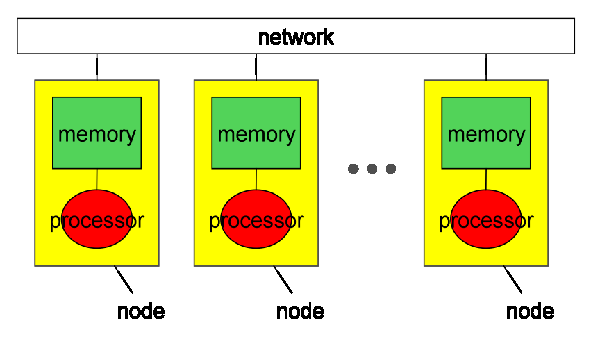
\includegraphics[width=12cm]{figs/Fig1.eps}
  \caption{Hardware model.}\label{fig1}
\end{myfigure}

\section{Execution Model}

An {\XMP} program execution is based on the Single Program Multiple Data
(SPMD) model, where each node starts execution from the same main
routine, and continues to execute the same code independently
(i.e., asynchronously), which is referred to as the {\it \Term{replicated
execution}}, until it encounters an {\XMP} construct.

%The basic execution model of {\XMP} is a Single Program Multiple Data
%(SPMD) model on distributed memory. In each node, a program starts from
%the same main routine.
%
%Unless the nodes encounter some {\XMP} directives, they executes the same
%code locally (i.e. asynchronously), which is referred to as
%{\it \Term{duplicate execution}}.

%An {\XMP} program begins as a single thread of
%execution in each node. 

%In this case, the
%program performs duplicate execution of the same program on local memory
%in each node.

%{\OMP} API can be used in order to make use of multicores in a node. In
%this specification, we define actions only when {\XMP} directives are
%executed one thread at a time.

A set of nodes that executes a procedure, statement, loop,
a block, etc. is referred to as its {\it \Term{executing node set}}, and is
determined by the innermost {\tt task}, {\tt loop}, or {\tt array}
directive surrounding it dynamically, or at runtime.
%
The {\it \Term{current executing node set}} is an executing node set of
the current context, which is managed by the {\XMP} runtime system on
each node.

%The initial ``current executing node set'' (or the {\it \Term{entire
%node set}}) at the beginning of the program execution is the set of all
%available nodes, which can be specified in an implementation-defined
%way (e.g. through a command-line option).

The current executing node set at the beginning of the program
execution, or {\it \Term{entire node set}}, is a node set that
contains all the available nodes, which can be specified in an 
implementation-defined way (e.g., through a command-line option).
%
%The entire node array is the node array if specified explicitly by the
%{\tt nodes} directive or an implicit one-dimensional node array if not.
%}

When a node encounters at runtime either a {\tt loop}, {\tt array}, or
{\tt task} construct, and is contained by the node set specified by the
{\tt on} clause of the directive, it updates the current executing node
set with the specified one and executes the body of the construct, after
which it resumes the last executing node set and proceeds to execute the
subsequent statements.

In particular, when a node in the current executing node set encounters a
{\tt loop} or an {\tt array} construct, it executes the loop or the array
assignment in parallel with other nodes, so that each iteration of the
loop or element of the assignment is independently executed by the node
in which a specified data element resides.

When a node encounters a synchronization or a communication directive,
synchronization or communication occurs between it and other nodes.
%
That is, such {\it \Term{global constructs}} are performed collectively
by the current executing nodes.
%
Note that neither synchronization nor communication occurs unless these
constructs are being specified.


\section{Data Model}

%By default, data declared in the program are allocated in each node and
%are referenced locally by threads executed in the node. 

There are two classes of data in {\XMP}: {\it \Term{global data}} and
{\it \Term{local data}}. Data declared in an {\XMP} program are local by
default.

Global data are distributed onto the executing node set by
the {\tt align} directive (see section \ref{sub:align}). Each fragment
of distributed global data is allocated in the local memory of a node in the
executing node set.
%
%Note that the ``address'' of a global data object is defined as that of its
%local section in each node and the results of any operations on such
%address are undefined.
%
%In contrast to a local-view programming model, a global-view programming
%model is a model in which programmers express their algorithm and data
%structure in their entirety, mapping them to the node set. The
%programmers describe the data distribution and the work mapping in order
%to express how to distribute data and share the workload among
%nodes. The variables in the global-view programming model appear as a
%shared memory spanning the nodes.

Local data comprises all data that are not global. They are replicated
within the local memory of each of the executing nodes.

%{\XMP} supports two models of data viewing: the global-view programming
%model and the local-view programming model. In the local-view
%programming model, accesses to data in remote nodes are performed
%explicitly by language extension for get/put operations on remote nodes
%with the node number of the target nodes, while reference to local data
%is executed implicitly.

A node can access directly only local data and sections of global data
that reside in its local memory.
%
To access data in remote memory, explicit communication must be
specified in ways such as global communication constructs and
coarray assignments.

%\underline{Description on memory layout to be added.}

In particular, in {\XMPF}, for common blocks that include any global
variables, it is implementation-defined what storage sequences they
occupy and how storage association is defined between two of them.

\section{Global-view Programming Model}

The global-view programming model is useful when, starting from a
sequential version of a program, the programmer parallelizes it in
data-parallel style by adding directives with minimum modification.
%
In the global-view programming model, the programmer describes the
distribution of data among nodes using the data distribution
directives.
%
The {\tt loop} construct assigns each iteration of a loop to the node
at which the computed data is located. 
%
The global-view communication directives are used to synchronize nodes,
maintain the consistency of shadow areas, and move sections of 
distributed data globally.
%
Note that the programmer must specify explicitly communications to make
all data references in the program local, and this is done using
appropriate directives.
%Note that the programmer must perform all computations that require data
%reference locally by any appropriate directives.

In many cases, the {\XMP} program according to the global-view
programming model is based on a sequential program, and it can produce
the same results, regardless of the number of nodes (Figure
\ref{fig2}).
%The global view provides a 
%programming model in which computation and data are distributed onto
%computation nodes.

There are three groups of directives for the global-view programming
model. Because these directives are ignored as a comment by the
compilers of base languages ({\Fort} and {\C}), an {\XMP} program can be
compiled by them to ensure that they run properly.

%an  {\XMP} program derived from a sequential program can preserve the
%integrity of the original program when the program is run sequentially. 

\subsubsection*{Data Mapping}

Specifies the data distribution and mapping to nodes (partially
inherited from HPF).

\subsubsection*{Work Mapping (Parallelization)}

Assigns a work to a node set. The {\tt loop} construct maps each
iteration of a loop to nodes owning a specific data elements. The {\tt
task} construct defines a set amount of work as a {\it \Term{task}}, and
assigns it to a specific node set.

\subsubsection*{Communication and Synchronization}

Specifies how to communicate and synchronize with the other compute
nodes. In {\XMP}, inter-node communication must be explicitly specified
by the programmer. The compiler guarantees that no communication occurs
unless it is explicitly specified by the programmer.

\begin{myfigure}
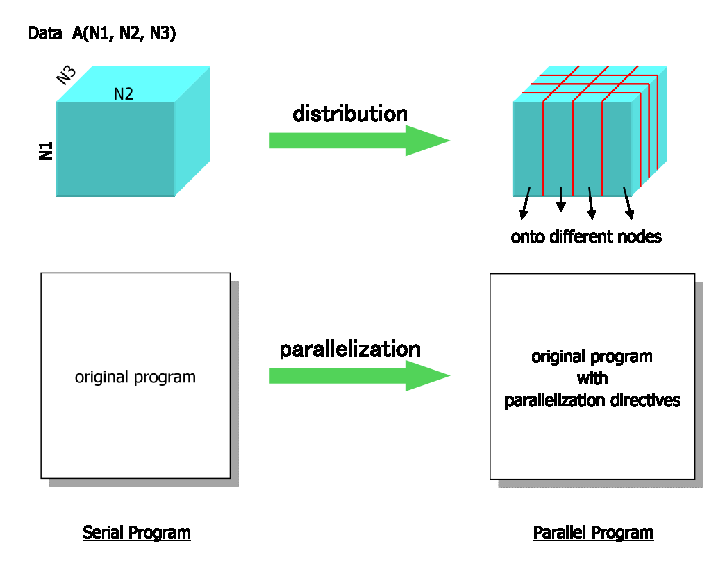
\includegraphics[width=12cm]{figs/Fig2.eps}
  \caption{Parallelization using the global-view programming model.}
\label{fig2}
\end{myfigure}

\section{Local-view Programming Model}

The local-view programming model is suitable for programs that
explicitly describe an algorithm and a remote data reference that are to
be executed by each node (Figure \ref{fig3}).
%Since MPI is based on the local-view model, the local-view programming
%model of {\XMP} has high interoperability with MPI.

For the local-view programming model, some language extensions and 
directives are provided. The coarray notation, which is imported from
{\Fort} 2008,
is one such extension, and can be used to specify which replica of a
local data is to be accessed. For example, the expression of {\tt
A(i)[N]} is used to access an array element of {\tt A(i)} located on the
node {\tt N}.
%
If the access is a reference, then a one-sided communication to get the
value from the remote memory (i.e., the {\it get} operation) is issued
by the executing node.
If the access is a definition, then a one-sided communication to put a
value to the remote memory (i.e., the {\it put} operation) is issued by
the executing node.

\begin{myfigure}
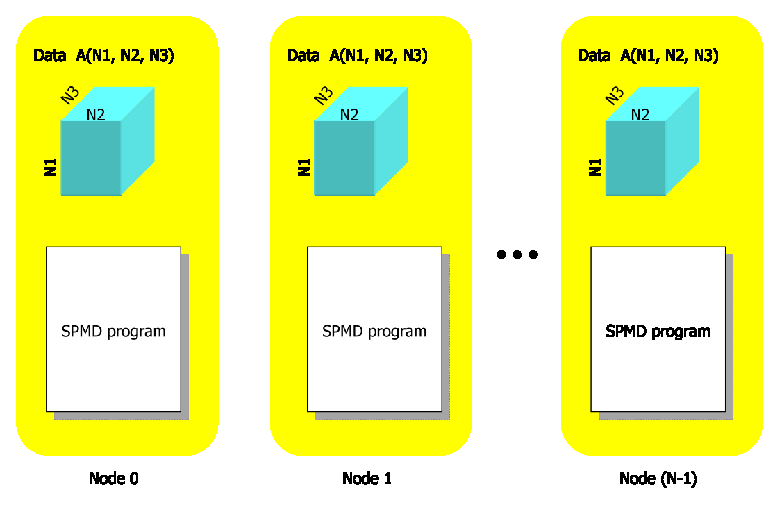
\includegraphics[width=12cm]{figs/Fig3.eps}
  \caption{Local-view programming model.}
\label{fig3}
\end{myfigure}

\section{Interactions between Global View and Local View}

In the global view, nodes are used to distribute data and works. In the
local view, nodes are used to address data in the coarray notation.
%
In application programs,
programmers should choose an appropriate data model according to the
structure of the program. Figure \ref{fig4} illustrates the global view
and the local view of data.

Data may have both a global view and a local view, and can be accessed
from either. {\XMP} provides some directives to give the local name
(alias) to the global data declared in the global-view programming model
to enable them to also be accessed in the local-view programming
model. This feature is useful to optimize a certain part of the program
by using explicit remote data access in the local-view programming
model.

\begin{myfigure}
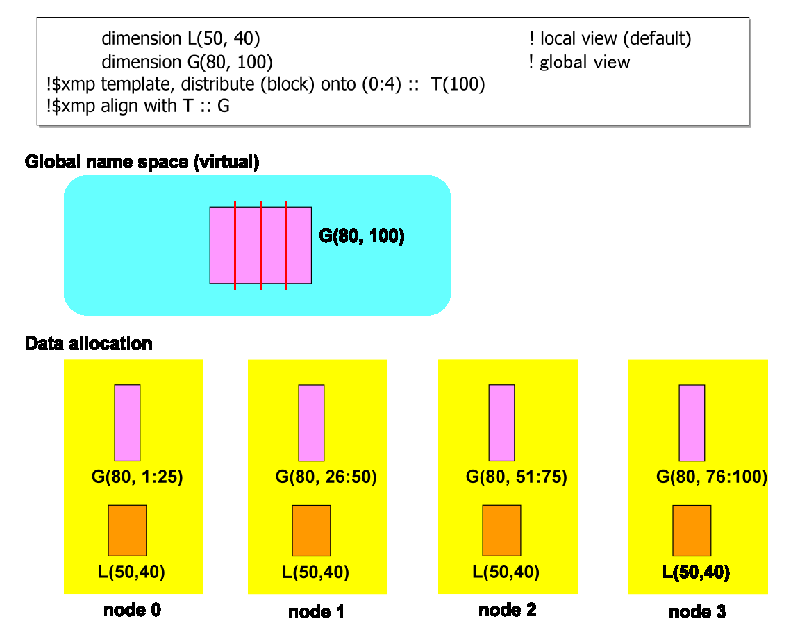
\includegraphics[width=12cm]{figs/Fig4.eps}
  \caption{Global view and local view.}
\label{fig4}
\end{myfigure}

\section{Base Languages}

The XcalableMP language specification is defined based on Fortran
and C as the base languages. More specifically, the base language of XcalableMP 
Fortran is Fortran 90 or later, and that of XcalableMP C is ISO C90
(ANSI C89) or later.

%\section{Execution model and task}
%
%
%In {\XMP}, a program begins as a single thread
%of execution in each node. The set of nodes when starting a program is
%referred to as the entire node set.
%
%A task is a specific instance of executable
%code and its data environment executed in a set of nodes. A task when
%starting a program in the entire node set is called an initial task. The
%initial task can generate a subtask, which is executed on a subset of the
%nodes by the {\tt task} construct. A set of nodes executing the same task is
%referred to as the set of executing nodes. If no {\tt task} construct is encountered, then a
%program is executed as a single task, and its executing nodes are the entire node set.
%
%If no directives are encountered, then a program is executed
%locally. When the same codes are executed, almost the same computation is
%performed in each node, which is referred to as duplicate execution. When the threads
%encounter a {\tt loop} construct or an {\tt array} construct, the specified
%loop is executed in parallel, so that each iteration is assigned to the
%node where the specified data element is located. 
%
%A new task is generated by
%the {\tt task} construct. A code in the {\tt task} construct is executed
%as a subtask executed in a specified node set. When a subroutine is
%called in the context of the task, the subroutine is executed on its
%executing nodes. 
%
%For synchronization and communication between nodes, a set of
%directives is provided. In the local-view programming model, coarray
%features are adopted for remote data reference. Note 
%that all synchronization and communication are specified explicitly by directives, and without such directives, no communications are
%executed implicitly by the compiler.
